\section{Design}
\label{sec:design}

%%\begin{figure}[t]
%%    \centering
%%    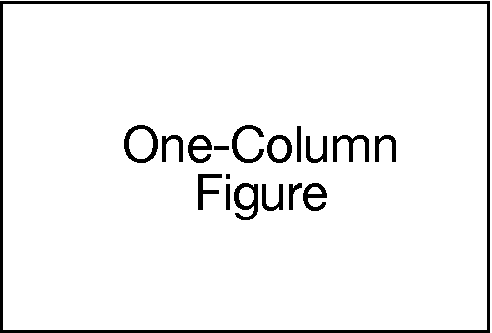
\includegraphics{diagrams/template.pdf}
%%    %
%%    \caption{High-level architecture.}
%%    %
%%    \label{fig:architecture}
%%\end{figure}

%% \parhead{Key management.}
%
In previous research, each function replica in a FaaS system would attest to a trusted key
server to obtain a shared key pair.
%
To eliminate this central, trusted dependency, \SystemName
uses decentralized key management with proxy re-encryption.
%
\begin{figure}
    \centering
    \includegraphics[page = 4, width=0.48\textwidth]{diagrams/slides.pdf}
    %
    \caption{\SystemName architecture.}
    %
    \label{fig:arch}
\end{figure}
%
As Figure~\ref{fig:arch} illustrates, the first instance of a function
generates a key pair and registers the public key in an untrusted registry,
along with an attestation report.
%
In \SystemName, that report will likely prove that the key was generated in an Oak
Trusted Execution Environment\@.
\color{red}TODO: move TEE stuff all to future work\color{black}
%
We'll discuss this future work in more detail in Section~\ref{sec:future}.
%As shown in Figure~\ref{fig:arch},
%the first instance of a function generates a key pair and registers the
%public key in an untrusted registry with an attestation report from an Oak
%TEE\@.
%attestation report that verifies the key was generated in an Oak TEE\@.
%
When a new replica is launched, the replica registers its own public key,
prompting the original instance to generate a re-encryption key.
%
%This enables any instance to encrypt messages for the original key pair,
%allowing independent scaling.
%
As a result, each function can encrypt messages for the original downstream
instance's public key, remaining independent of that function's scaling.



%% \textbf{Compilers project proposal}

In this section we'll overview the design of the \SystemName system.
%%%
%%First, in section \ref{sec:samba}, I'll describe the proposed \SystemName design.
%%%
%%Then, in section \ref{sec:optimization_design} we'll discuss proposed compiler optimization and general optimizations for the \SystemName system. Finally, in section \ref{sec:eval} we'll cover the means by which I'll evaluate the relative success (or failure) of those performance improvements.
%%%
\SystemName applies proxy re-encryption to Function as a Service (FaaS) applications.
%
We implement it as an extension to Knative Serving\footnote{\url{https://knative.dev/docs/serving/}}, an open-source cloud technology that can function as a FaaS orchestrator.
%
Knative Serving is a Kubernetes-based platform that enables developers to deploy and manage serverless applications.
%
Using their existing Knative Serving infrastructure, we can add \SystemName's proxy re-encryption capabilities to functions deployed on Knative.
%
Knative functions have \texttt{QueueProxy} sidecar containers that can be used to perform instance-level re-encryption operations on the function's behalf.



We implement \SystemName-Lite, a simplified proof-of-concept for the proxy re-encryption scheme applied to FaaS.
%
To understand how \SystemName-Lite works, I'll describe a simple example where we have a function with a maximum of two replicas, Alice and Bob.
For the sake of consistency we'll call the FaaS provider/orchestrator Proxy.
For simplicity in this explanation, we'll assume not only Proxy, but also Alice and Bob are always running, which defeats the entire purpose of FaaS, but doesn't effect our analysis of the cryptographic operations.
We assume that Alice's public key will be known by any prospective clients wishing to run the function, since she is the leader replica, so Proxy will advertise her public key as the public key of the function.
Requests destined for the function are encrypted under Alice's public key, and sent by some Sender to Proxy.
Proxy then load balances, determining if Alice can currently accept a request.
If so, Proxy forwards the request to Alice, who can decrypt it with her private key, and send her response to the Proxy, who forwards it to Sender.
If not, Proxy selects an availible replica, in this case Bob, and requests a re-encryption key from Alice to Bob (if one hasn't already been made).
Proxy then re-encrypts the request to Bob, forwards the request to Bob.
Bob decrypts, and responds to Proxy, who forwards that response to Sender.
The decryption operation for a re-encrypted message is different than a normal RSA decryption, which we'll touch on more in section~\ref{sec:PRE}.

%% \subsection{Optimization}
%% \label{sec:optimization_design}
%% 
%% The performance impact of adding proxy re-encryption to an otherwise un-encrypted program is no secret.
%% The AFGH authors aren't shy about this, but do mention that if they had gone to greater lengths to select proper compiler optimizations, these effects could be reduced.
%% \cite{afgh}
%% That is the motivation for this proposal.
%% With our proxy re-encryption implementation written in Go, we have access to a compiler with many optimizations already built in, and a rich ecosystem of open source extensions.
%% The primary contribution of this project will be, through theoretical research, as well as trial and error, determining what set of optimizations for the Go compiler produce the best results for proxy re-encryption in the Samba system.
%% 
%% Beyond the possible compiler optimizations, we will make sure to do another simple optimization at the code level.
%% If we were to write the least amount of code possible to implement proxy re-encryption within Samba, that would probably involve the initial replica generating re-encryption keys to re-encrypt messages to itself, so we wouldn't have to code anything for that "base case."
%% The optimization here would be to simply code specifically for the case where the request is load balanced to the initial replica, and skip the re-encryption key generation, and re-encryption steps.
%% This will limit the cryptographic operations performed to those that are absolutely necessary.
%% 
%% \subsection{Evaluation}
%% \label{sec:eval}
%% 
%% Knative and the Samba extension are both written in Go.
%% Among the many benefits of the Go Programming Language is its standard library, which contains many idiomatically written packages for tasks developers need to perform frequently.
%% In our case, we'll make extensive use of the "testing" package, and specifically its benchmarking support.
%% This will be most helpful for testing the effectiveness of our optimizations on the \texttt{alice}, \texttt{bob}, and \texttt{proxy} binaries within the proof-of-concept \SystemName-Lite portion of the project.
%% 
%% Additionally, Knative itself offers a number of ways to benchmark components in its distributed system.
%% \cite{knative_serving}
%% We will use these tests to compare the performance of Knative's Autoscaling Sample App without the Samba extension vs. with the Samba extension.
%% \cite{autoscale_sample_app_go}


%%
%In previous research, to ensure each function replica used the same key pair,
%each replica would attest to a trusted key server, which then provided the
%correct key pair based on the replica's attestation measurement.
%%
%To remove this reliance on centralized, trusted infrastructure, \SystemName
%employs a decentralized key management system using proxy re-encryption.
%%
%\begin{wrapfigure}{l}{0.5\textwidth}
%    \centering
%    \includegraphics[page = 4, width=0.48\textwidth]{diagrams/slides.pdf}
%    %
%    \caption{\SystemName architecture.}
%    %
%    \label{fig:arch}
%\end{wrapfigure}
%%
%As Figure~\ref{fig:arch} illustrates, the initial instance of the function
%generates a key pair and registers the public key in an untrusted registry,
%along with an attestation report that verifies the key was generated in an Oak
%TEE\@.
%%
%When the FaaS platform launches a new replica of the function, the replica
%generates and registers its own public key.
%%
%This triggers the FaaS platform to request the initial function instance to
%produce a re-encryption key for the new replica.
%%
%As a result, each function can encrypt messages for the original instance’s
%public key, remaining independent of the function's scaling.



%%\begin{table}[t!]
%%    \small
%%    \caption{Time (s) to Re-encrypt a Bucket of Size 1G}
%%    \label{tab:enclave-overhead}
%%    \centering
%%    \begin{tabular*}{0.48\textwidth}{|r|@{\extracolsep{\fill}}r|r|}
%%        \hline
%%        \textbf{Environment}  &\textbf{Akeso}  &\textbf{Strawman}  \\
%%        \hline
%%        \textbf{Confidential VM}    &47.231  	 &118.239  \\             
%%        \textbf{Non Confidential VM}        &44.907	    &109.366 \\            
%%        \hline 
%%    \end{tabular*}
%%\end{table}

%% \textbf{adwait}
%% 
%% There are a number of open source projects for various parts of the project that we will be extending.
%% 
%% \subsection{Function Runtime}
%% We performed all development and testing on an AMD-SEV SNP machine, to later take advantage of Trusted Execution Environment features.
%% We have not yet enabled these features in the course of development.
%% We ported an open source proxy re-encryption library from C to Rust in order to be callable from within the later boot stages of the Oak Restricted Kernel.
%% The kernel extension itself is still a work in progress.
%% There is a lot to sort through to determine where exactly in the boot stages would be the best place to perform re-encryption and decryption
%% to be able to work with the data.
%% 
%% \subsection{FaaS Orchestration}
%% Function as a Service paradigms are implemented differently by different platforms.
%% Amazon Lambda, Google Cloud Functions, and Azure Functions are all well-known and closed source, all with (presumably) completely different architectures.
%% 
%% The open source FaaS landscape is no more homogenous than its corporate counterpart.
%% Additionally, some are partially open source, with certain paywalled features, and others use deprecated dependencies which makes setup a non-trivial problem.
%% This was a major hurdle for development, and battling the idiosyncracies of these FaaS frameworks accounts for much of the progress (or lack thereof) made on this project.
%% 
%% \subsubsection{Firecracker}
%% Firecracker is partially open source, and disbatches requests to networks of MicroVMs.
%% Since it doesn't support custom kernels out of the box, and a lot of the code is written with MicroVM specific APIs, extending this project to accomodate the Oak Restricted Kernel for SAMBA would amount to basically a full rewrite.
%% 
%% \subsubsection{OpenFaaS}
%% OpenFaaS, perhaps misleadingly, is not fully open source.
%% Components such as the load balancer that creates function replicas are only availible as binaries, and therefore the modifications that we need to make are not possible with OpenFaaS.
%% 
%% \subsubsection{OpenWhisk}
%% OpenWhisk is fully open source, and is used in a variety of recent papers. That said, the repository seems barely maintained in 2024, and older versions of Java (Java 8), Docker, and Ubuntu may be required to cohesiveliy run it.
%% Investigations to that effect are another significant contributor to delay in this project.
%% We anticipate continuing efforts, potentially of a known working fork from a researcher who has used OpenWhisk successfully in recent years.
%% Also, I will re-double my efforts following and modifying few-yearold open source documentation to get development up and running, by emulating all dependencies as closely as possible.
%% 
%% \subsubsection{Open Function}
%% Open Function is another open source function orchestrator, which we will look into as an implementation option.
%% 
